\documentclass[main]{subfiles}

\begin{document}
  \begin{lect}{2019-10-28}
      %\begin{reminder}
          %рисунок1 с поверхностью
      %\end{reminder}
      \subsection{Соприкасающийся параболоид. Классификация точек поверхности}
      <<Введем нового героя>>
      \begin{Definition}
          %рисунок2 с пр-вом и точкой A
          \[A \text{ - точка на пов-ти}\]
          \begin{figure}[H]
              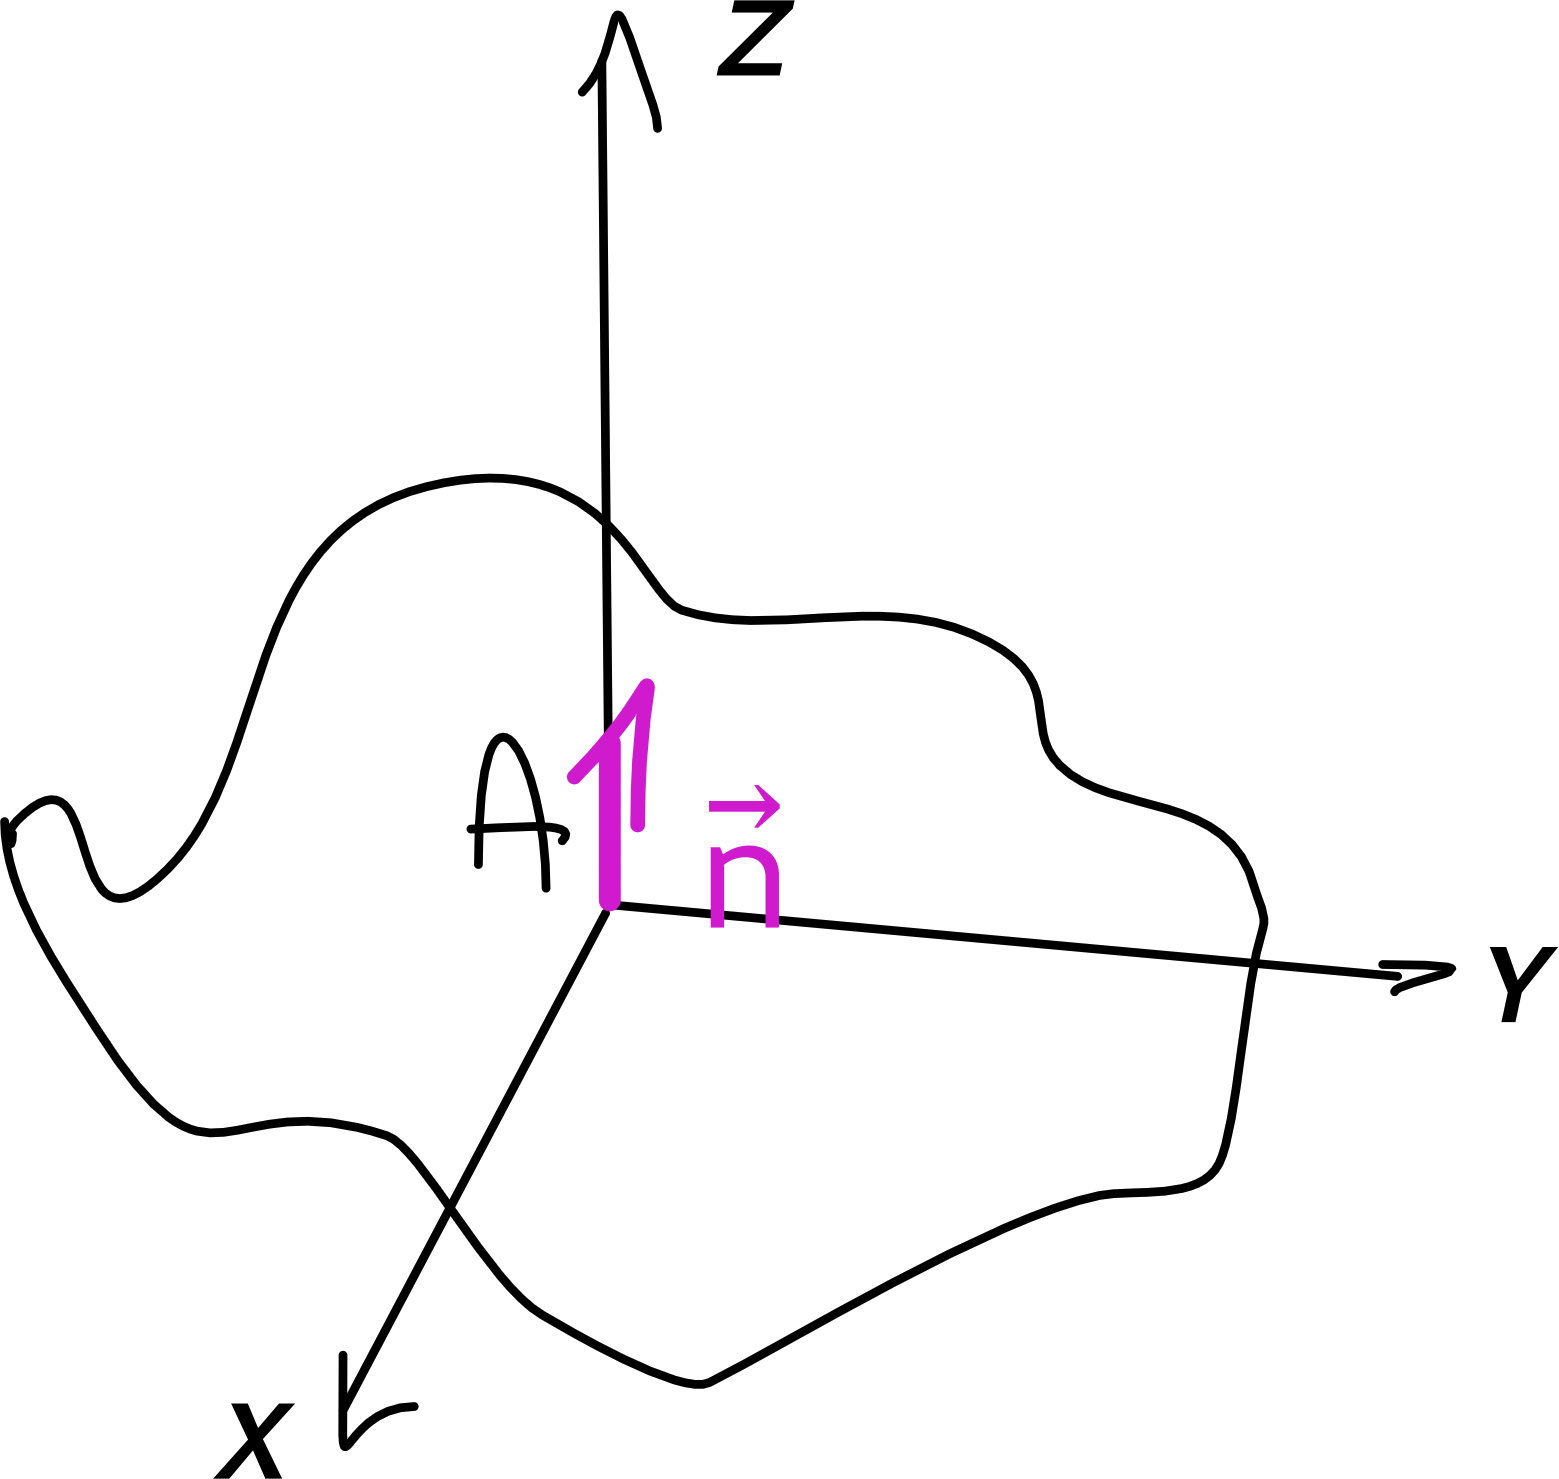
\includegraphics[width=3.5cm]{pics/8_2.png}
              \centering
          \end{figure}
          \[\Ra \text{ в окр. } A \text{ поверхность задается } z = f(x, y)\]
          \[x_0 = 0 \q y_0 = 0 \q z_0 = f(x_0,\ y_0) = 0\]
          Разложим $z=f(x, y)$ по ф. Тейлора
          \[z = f(x, y) = f(x_0, y_0) + f_x(x_0, y_0)x + f_y(x_0, y_0)y + \]
          \[\frac{1}{2}(f_{xx}(x_0, y_0)x^2 +
          2f_{xy}(x_0, y_0) )xy + f_{yy}(x_0, y_0)y^2) \]
          \[f_x(0, 0) = 0 \qq f_y(0, 0) = 0\]
          \[r(v, u) = \begin{cases}
              x = u\\
              y = v\\
              z = f(u, v)
          \end{cases} \qq r_u = \begin{pmatrix}
              1\\
              0\\
              f_u
          \end{pmatrix} \qq r_v = \begin{pmatrix}
              0\\
              1\\
              f_v
          \end{pmatrix}\]
          \[r_u \text{ и } r_v \text{ - лежат в кас. плоск, а это } OXY\]
          \[z = \underbracket{\frac{1}{2}(f_{xx}(0, 0)x^2 + 2f_{xy}(0, 0)xy +
              f_{yy}(0, 0)y^2) }_{\text{пов-ть 2 порядка}} +
          o(x^2 + y^2)\]
          \[z = Ax^2 + 2Bxy + Cy^2\]
          \[z = Ax^2 + Cy^2 \text{ можем поворотом привести к этому}\]
          Это может быть: \\
          \begin{matrix}
              &\text{- эллиптич. параболоид}&  A, C \text{  - одного знака}\\
              &\text{- гипербол. параболоид}&  A, C \text{ - разных знаков}\\
              &\text{- параболический цилиндр}&\q  A = 0, \q C \neq 0 \text{  или наоборот}\\
              &\text{- плоскость}& A = 0,  C = 0
          \end{matrix}
         %хахахааххахааххахаххахаххахаха
      \end{Definition}

      \begin{definition}
          Точка A наз. элиптической, если соприкас. параболоид - элипт.\\
          А - гиперболическая, если соприкас параболоид - гиперб.\\
          А - парабол., если соприкас параб - параб. цилинд или плоскость
      \end{definition}

      \begin{definition}
          Точка А наз. точкой округления (омбилическая), если сопр. параб. - пар. вращения
      \end{definition}

      \begin{definition}
          Точка A - точка уплощения, если соприкас. параб - плоскость
      \end{definition}

      \subsection{Совпадение нормальных кривизн поверхности и соприкасающегося параболоида}
      \begin{Theorem}
          \[\RNumb{1} \text{ и } \RNumb{2} \text{ формы в точке }A
          \text{ у поверхности и параболоида совпадают}\]
          %рисунок3
          \begin{figure}[H]
              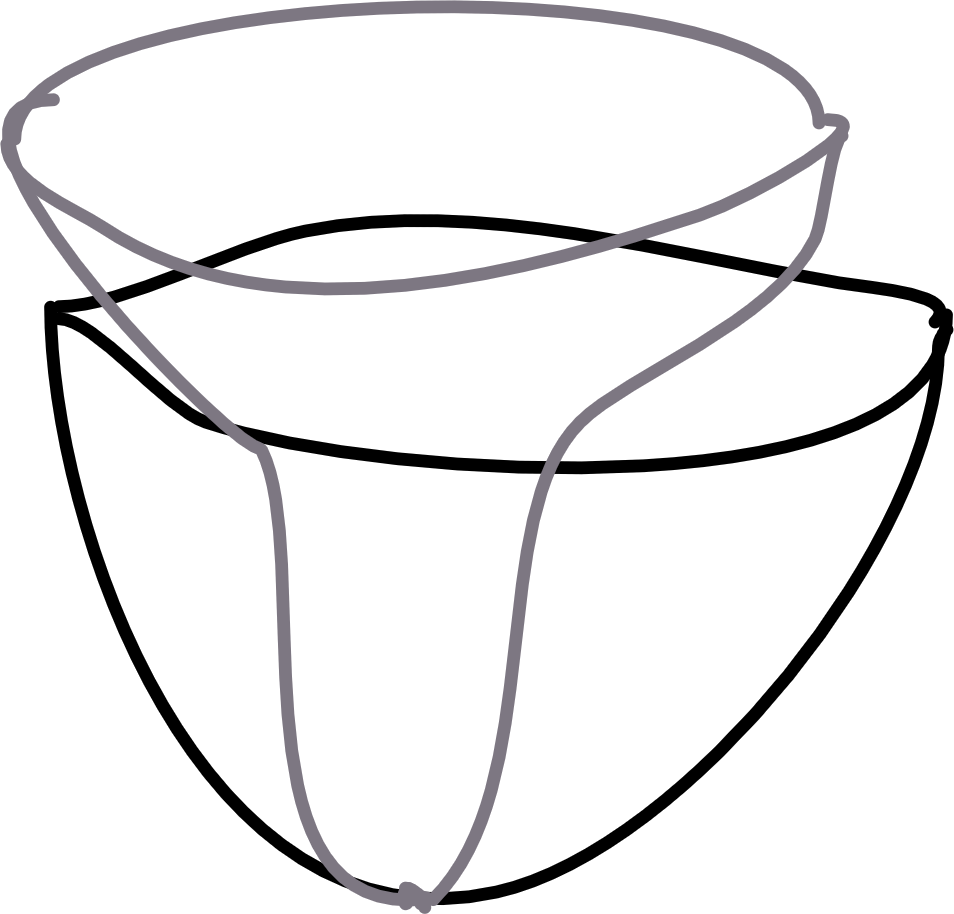
\includegraphics[width=6cm]{pics/8_4.png}
              \centering
          \end{figure}

          В параметризации $\begin{cases}
              x = u\\
              y = v\\
              z = f(u, v)
          \end{cases}$

          \begin{proof} %тут какая-то фигня
              очевидно\\
              Давайте поймем, от чего зависят $E, F, G, L, M, N$?\\
              от $\ol{r}_u, \ \ol{r}_v, \ \ol{r}_{uu}, \ \ol{r}_{uv}, \ \ol{r}_{vv}   $
          \end{proof}

          \begin{consequence}
              Норм. кривизны у поверх-ти и соприкас. параб совпадают
          \end{consequence}

          \begin{definition}
              Главные кривизны $k_1$ и $k_2$
              \[\vec{a} \text{ - направление в кас. плоск}\]
              \[\ol{k}_{\vec{a}} \text{ - нормальная кривизна}\]
              \[k_{\vec{a}} \text{ - норм. кривизина в напр. } \vec{a} \]
              \[\ol{k}_{\vec{a}} = k_{\vec{a}} \overline{n}  \]
              \[k_1 = \min_{\vec{a}} k_{\vec{a}}  \qq k_2 = \max_{\vec{a}} k_{\vec{a}}   \]
          \end{definition}
      \end{Theorem}

      \begin{Definition}
          \[\vec{a}_1 \text{ и } \vec{a}_2 \text{, соотв } k_1 \text{ и } k_2 \text{ наз.
          главными направлениями}\]
      \end{Definition}

      \begin{Utv}
          \[\vec{a}_1 \perp \vec{a}_2 \text{(докажем позже)}\]
      \end{Utv}

      \begin{Definition}
          \[K = k_1 \cdot k_2 \text{ - гауссова кривизна}\]
          <<Главный герой всего нашего курса>>
      \end{Definition}

      \begin{Properties}
          \[\begin{matrix}
              K > 0 &\rla& A \text{ - эллипт типа}\\
              K < 0 &\rla& A \text{ - гиперб. типа }\\
              K = 0 &\rla& A \text{ - параб. типа}
          \end{matrix}\]
      \end{Properties}

      \begin{Utv}["Блистательная теорема Гаусса"]
          \[K \text{ - инвариант относительно изометрии пов-ти}\]
      \end{Utv}

      \begin{Definition}
          \[H = \frac{k_1 + k_2}{2} \text{ - средняя кривизна}\]
          \ul{Смысл:} В мыльных пленках (незамкн.) средняя кривизна = 0
          %рисунок4
          \begin{figure}[H]
              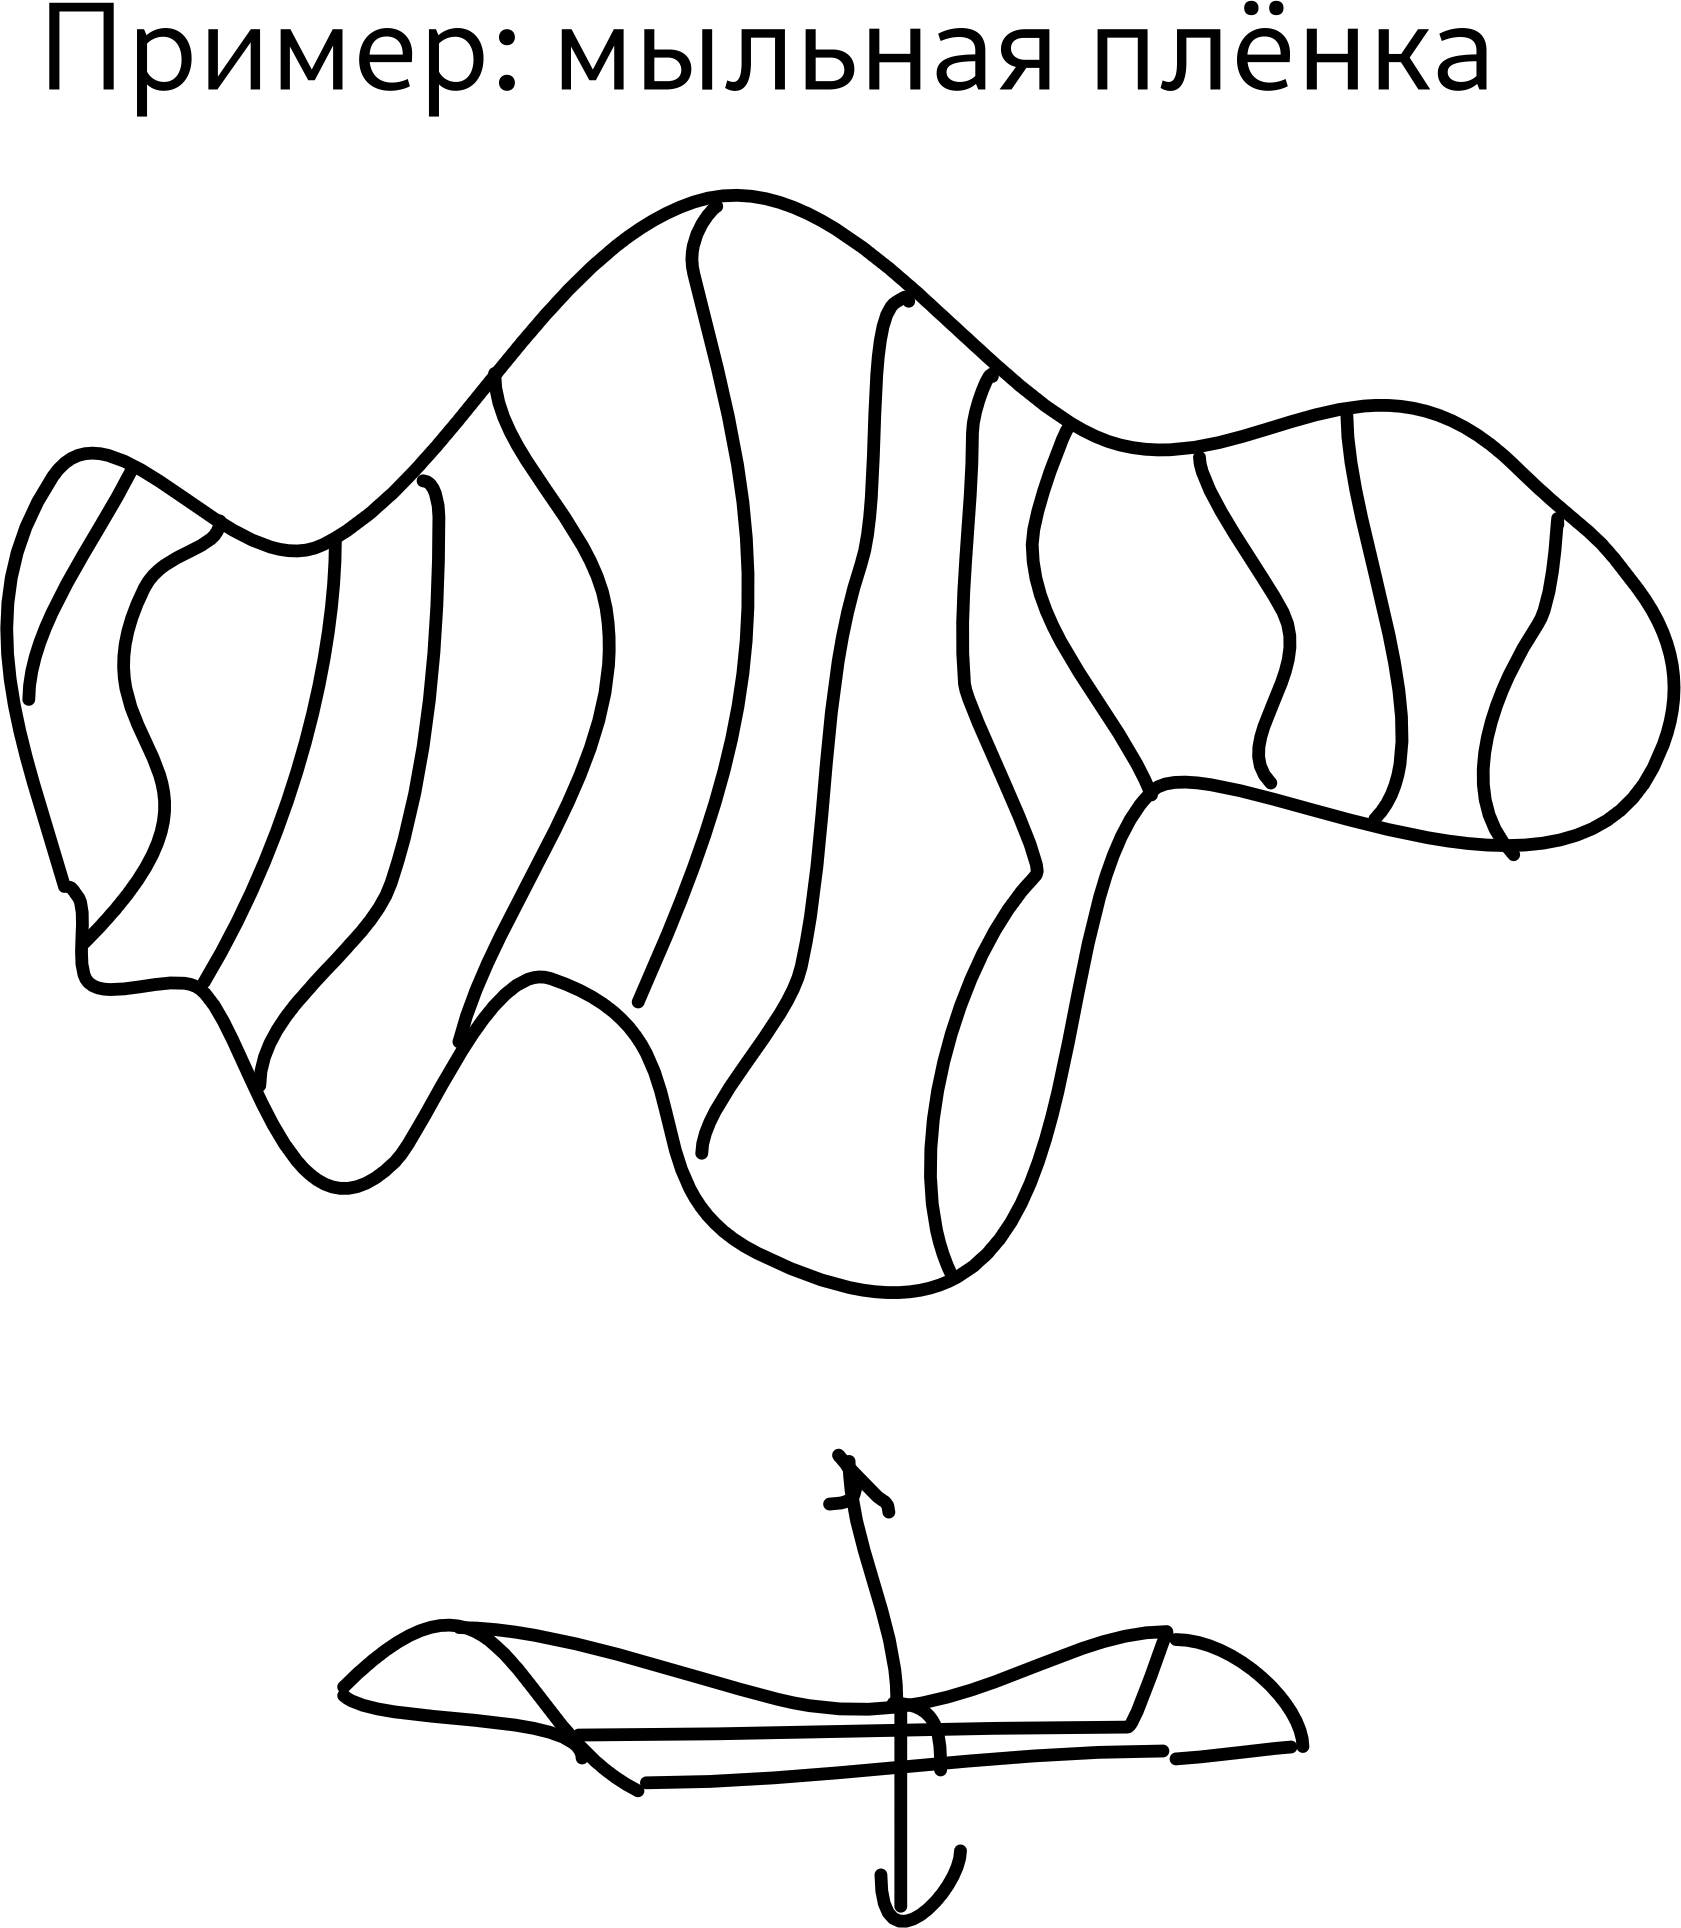
\includegraphics[width=5cm]{pics/8_5.png}
              \centering
          \end{figure}

      \end{Definition}

      \subsection{Теорема Эйлера}
      \begin{Theorem}[Эйлера]
          \[k_{\vec{a}} = k_1 \cos^2 \Theta + k_2 \sin^2\Theta \]
          \[\text{где } k_1, k_2 \text{ - гл. кривизны, } \Theta \text{ - угол между
          напр. } \vec{a} \text{ и } \vec{a}_1\]
      \end{Theorem}

      \begin{Proof}
          \[ z = Ax^2 + C y^2 \text{ - сопр. парабол.} \]
          \[\vec{a} = (\cos \Theta;\ \sin \Theta) \text{ - направление}\]
          %рисунок плоск с \vec{a}
          \[\begin{cases}
              x = t\cos\Theta\\
              y = t\sin\Theta\\
              z = Ax^2  + Cy^2 = t^2(A \cos^2\Theta + C \sin^2 \Theta)
          \end{cases}\]
          \[\vec{r}'(t) = \begin{cases}
              \cos \Theta\\
              \sin \Theta\\
              2t(A\cos^2\Theta + C\sin^2\Theta)
          \end{cases}\]
          \[r''(t) = \begin{cases}
              0\\
              0\\
              2(A\cos^2\Theta + C\sin^2\Theta)
          \end{cases}\]
          \[k = \frac{\abs{r'(t_0) \times r''(t_0)}}{\abs{r'(t_0)}^{3/2} }\]
          \[t_0 = 0\]
          \[r'(t_0) = \begin{pmatrix}
              \sin \Theta\\
              \cos \Theta\\
              0
          \end{pmatrix} \qq \abs{r'(t)} = 1\]
          \[r''(t_0) = \begin{pmatrix}
              0\\
              0\\
              2(A\cos^2 \Theta + C\sin^2 \Theta)
          \end{pmatrix}\]
          \[\abs{r''(t_0)} = 2\abs{A\cos^2\Theta + C\sin^2\Theta}\]
          \[r'' \perp r'\]
          \[\text{В данном случае } k = \abs{r''(t_0)} = 2\abs{A\cos^2 \Theta +
          C\sin^2 \Theta}\]
          \[k_{\vec{a}} = \pm k \q\text{(от сонапр. с } \vec{n}) \]
          \[k_{\vec{a}} = 2(A\cos^2 \Theta + C\sin^2 \Theta) \]
          Хотим теперь найти минимум и максимум этой штуки, но не хотим брать произв.
          \[k_{\vec{a}} = 2(A\cos^2\Theta + C(1 - \cos^2 \Theta)) = 2C + \cos^2 \Theta
          (2A - 2C)\]
          При $A = C$ \q A - точка округл.
          \[\letus A > C\]
          \[\max k_{\vec{a}} \text{ достиг при } \Theta = 0 \q(\text{или } \pi) \]
          \[k_1 = 2C + 2A - 2C = 2A\]
          \[\min k_{\vec{a}} \text{ при } \frac{\pi}{2} \q(\text{или } -\frac{\pi}{2}) \]
          \[k_2 = 2C\]
      \end{Proof}

      \begin{consequence}[1]
          Пов-ть задана ур-ем $z = f(x, y)$
          \[f(0, 0) = 0 \qq f_x(0, 0) = 0 \qq f_y(0, 0) = 0 \qq f_{xy}(0, 0) = 0 \]
          \[\Ra k_1 = f_{xx}(0, 0) \q k_2 = f_{yy} (0, 0)\]
          \[\text{ (или наоборот мы
          рассматривали только } A > C)\]
      \end{consequence}

      \begin{consequence}[2]
          Главные напр $\perp$
      \end{consequence}
  \end{lect}
\end{document}
